\documentclass{70_styles/svproc}

\usepackage{url}
\usepackage{biblatex}
\usepackage{graphicx}
\usepackage{amsmath,amssymb,amsfonts}
\usepackage{subcaption}

\bibliography{70_styles/bibtex/sn-bibliography}

\def\UrlFont{\rmfamily}
\begin{document}
\mainmatter 

\title{Edge Map Extraction of High Resolution Facial Images}
\titlerunning{Edge Map Extraction of High Resolution Facial Images}

\author{Harshit Timmanagoudar \and Gandra Sai Krishna \and Anirudh Koti \and Harsh Jolad \and Preethi P}
\authorrunning{Harshit Timmanagoudar et al}
\institute{Department of Computer Science, PES University, Bangalore, 560085, Karnataka, India,\\
\email{harshit.utd@gmail.com},
\email{saikrishnag03@gmail.com},
\email{ani040702@gmail.com}
\email{harshjolad@gmail.com},
\email{preethip@pes.edu}}

\maketitle 

\begin{abstract}
This work focuses on edge detection, a vital task in several fields, such as computer vision, image processing, and pattern recognition. Since exact facial analysis and recognition have numerous applications in areas like bio metrics, surveillance, and human-computer interaction, this study's focus is specifically on obtaining precise edge maps of facial pictures with exceptional resolution. Several essential processes are carried out in order to produce accurate edge maps. In order to lessen noise and attenuate the very low level features in high resolution photographs, a smoothing operation is first conducted. Utilising a variety of edge detection methods, such as directional gradients and cumulative gradient magnitude, variations in pixel intensities along various directions are examined. The Zhang Suen technique, renowned for its efficiency in thinning binary pictures, is used to remove extraneous pixels from the discovered edges to further refine them. By maintaining only the necessary boundary information, this phase ensures that the edge maps produced are more accurate. According to subjective and comparative evaluations and the outcomes of applying the algorithm to face photos from various datasets, the suggested approach is suitable for building edge maps of facial photographs with high resolution as well as low resolution.
\keywords{Edge detection, Facial images, Directional gradients, Zhang Suen Algorithm}
\end{abstract}

\section{Introduction and Related Work}
Identifying and locating boundaries or edges inside an image is the goal of the fundamental image processing technique known as edge detection. For a number of reasons, it is crucial to detect edges in facial images.  First, edges offer crucial hints regarding the structure and contour of the face, facilitating precise face recognition and identification. Edge detection makes it easier to localise these regions for later analysis by extracting the borders of face features like the eyes, nose, and mouth. Second, by simplifying the representation of the facial structure, edge detection aids in the reduction of the complexity of facial images. Edge detection permits the concentrate on critical features rather than having to cope with a vast number of pixels, increasing computing performance and requiring less memory.

There are several uses for edge detection in facial photographs. Edge information can be utilised in face recognition algorithms to handle position fluctuations, align faces, and enhance matching accuracy. Edge detection facilitates the extraction of expressive regions and helps with emotion recognition in facial expression analysis. Edge detection also aids in the recognition of facial landmarks, such as the eyes, brows, and mouth, which is useful in applications like facial animation, virtual reality, and character modelling.

Early pioneering methods for edge detection involve techniques such as Sobel \cite{996}, Prewitt \cite{6100495}, zero-crossing \cite{1980} \cite{4767769}, Scharr \cite{levkine2012prewitt}, Canny edge detection \cite{4767851} and Improved Canny edge detection \cite{6885761}. Structured Forests for Fast Edge Detection \cite{6975234} is a research work that introduces an efficient edge detection method based on structured random forests, enabling real-time performance and robustness in challenging imaging conditions. Several notable methods have explored the application of convolutional neural networks (CNNs) for edge detection. One such method, Holistically-Nested Edge Detection \cite{xie2015holisticallynested}, proposed a deep CNN architecture trained end-to-end to generate multi-scale and multi-level edge predictions. The method titled DeepEdge \cite{bertasius2015deepedge} employed a multi-scale and multi-level CNN architecture to capture local and global information for accurate contour detection. DeepContour \cite{7299024}, improved contour detection by incorporating a positive-sharing loss function in a deep CNN, emphasizing high-level semantic information. Generative Adversarial Networks \cite{chen2020edge} have also been explored for extracting edge maps. CannyGAN \cite{8803828} combined generative adversarial networks (GANs) with a traditional edge detector to generate high-quality edge maps. CSCNN (Convolutional Spatial CNN) \cite{9407182} is a deep learning architecture designed for edge detection that incorporates spatial information and achieves high-quality edge predictions.
These methods demonstrate the diverse approaches in leveraging CNNs for edge detection, aiming to enhance accuracy and efficiency in extracting edge information from images. The proposed algorithm from the research work \cite{6460720} demonstrate effective performance in identifying edges of facial images, challenges persist when dealing with high-resolution images. The abundance of information and noise within high-resolution images can hinder the production of pleasing edge maps. This limitation arises because not all the information and noise contribute to the desired edge map, hindering further analysis. Therefore, the primary objective of producing an edge map for high-resolution images is to effectively highlight the facial outline while maintaining a balance with low-level details. To address this, our proposed methodology employs a series of steps. These steps encompass smoothing techniques to reduce noise, the detection of strong and weak edges, merging of the identified edges, and refining processes to attain the desired result. 

Section II of the research work provides a detailed description of the proposed algorithm for edge detection in facial images. It explains the methodology and steps involved in effectively highlighting the facial outline. In section III, a comparative analysis is conducted to select the optimal sigma value for the smoothing technique, an important component of the algorithm. Section IV focuses on performance measurement and evaluation. The dynamism of the proposed algorithm is checked by running it on different dataset containing both low resolution as well as high resolution images. A comparative study with the Canny edge detection and HED algorithms is conducted. Subjective analysis by human evaluators is also included to assess the visual quality and user perception of the edge maps. These sections collectively provide insights into the algorithm's methodology, parameter selection, and performance evaluation, demonstrating its potential for improving edge detection in facial images.

After running the algorithm on a diverse set of high-resolution facial images, the results obtained are exemplified in Figure 1. These results showcase the effectiveness of the algorithm in accurately detecting and highlighting the facial edges. The subsequent section provides a detailed walkthrough of the algorithm's steps, aiming to replicate the desired outcomes demonstrated in Figure 1. By following this detailed explanation, it becomes possible to achieve edge detection results that closely resemble those presented in Figure 1, further validating the algorithm's capabilities.

\begin{figure}
     \centering
     \begin{subfigure}[b]{0.2\textwidth}
         \centering
         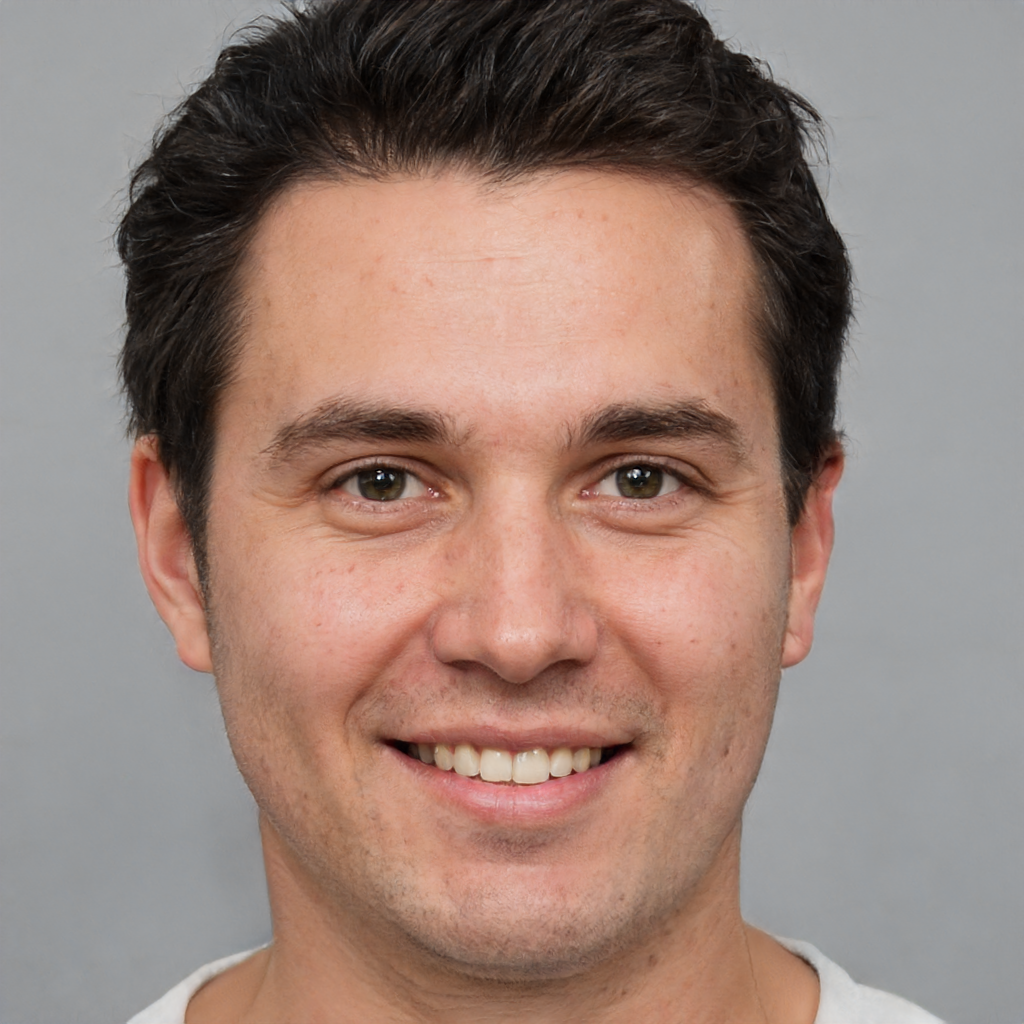
\includegraphics[width=\textwidth]{70_figures/seed0270.png}
     \end{subfigure}
     \begin{subfigure}[b]{0.2\textwidth}
         \centering
         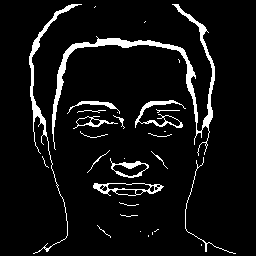
\includegraphics[width=\textwidth]{70_figures/seed0270_EM.png}
     \end{subfigure}
     \caption{Desired output image}
\end{figure}

\section{Algorithm}

\subsection{Smoothing}

A conventional image's energy is predominantly concentrated in its low-frequency components because surrounding pixels have strong spatial correlation with one another. Wide band random noise frequently contains energy that is spread more equally across the frequency range. Low pass filtering keeps the low-frequency components while reducing the high-frequency components to significantly reduce noise while improving the image for further processing of edge detection.

Due to the high resolution of the photos under consideration, a smoothing method must be used to produce the requisite edge maps. This is especially true for facial images since they frequently include a lot of fine details, including hair strands, dark patches, and other small characteristics, that might hide or complicate the boundaries. These particulars might affect the edge map's accuracy and clarity without the smoothing step, making it challenging to extract the necessary information. Therefore, smoothing techniques must be used to help lessen the impact of these extraneous details in order to effectively capture the images' key characteristics and produce high-quality edge maps.

The facial image is smoothed in the proposed technique using a Gaussian low-pass filter, as shown in (1). 

\begin{equation}
    h(x,y)\ =\ e^{-(x^2 + y^2)/2.\pi.\sigma^2}
\end{equation}

The Gaussian kernel size is governed by $\sigma$, which is the standard deviation. Greater values of $\sigma$ result in more picture blurring, which reduces noise by a greater amount. However, larger $\sigma$ also means that finer edges are excluded and only larger edges are detected.

Thus, removing high frequency noise components from the image requires an optimal value of $\sigma$. $\sigma$ is initially given a value of 2 for the experiments.

The result of the operation can be visualized with the help of Fig 2.

\begin{figure}
     \centering
     \begin{subfigure}[b]{0.2\textwidth}
         \centering
         
\includegraphics[width=\textwidth]{70_figures/seed1830.png}
     \end{subfigure}
     \begin{subfigure}[b]{0.2\textwidth}
         \centering
         
\includegraphics[width=\textwidth]{70_figures/smoothened-seed1830.png}
     \end{subfigure}
     \caption{Resultant image obtained from performing smoothing operation on high resolution image with $\sigma$ value equal to 2.}
\end{figure}

\subsection{Directional Gradients}
Selecting the appropriate convolution kernel with the ideal size and direction is one of the crucial phases in recognising edges in facial images. Wide convolution kernels often have the tendency to reduce noise and minor spurious peaks. By giving closer points more weight than faraway ones, weighted convolution kernels have been shown to minimise noise while keeping the true edge peaks to some extent \cite{Kanade-1977-15584}.

We combine horizontal and vertical directional filters in our technique to calculate directional derivatives. Let the smoothed picture from the previous step be represented by the 2-D sequence $f(i, j)$. Let the partial derivatives along the horizontal and vertical axes be represented by $\frac{\partial f(x, y)} {\partial x}$ and $\frac{\partial f(x, y)} {\partial y}$, respectively. Some kind of discrete difference can be used to represent these partial derivatives. The horizontal and the vertical discrete differences are given by the equations (2) and (3) respectively.

\begin{equation}
    f_x(i, j) = f(i, j) * h_x(i, j)
\end{equation}

\begin{equation}
    f_y(i, j) = f(i, j) * h_y(i, j)
\end{equation}

where $h_x$ and $h_y$ in the equations (2) and (3) represent the horizontal and the vertical impulse response filters respectively. Points within two pixel intervals in addition to the directly adjacent pixels when computing the discrete differences are considered. Better noise suppression results from doing so, generally. 

Gradients in both horizontal and vertical directions have so far been calculated. This tends to properly identify edges that run vertically and horizontally, but in order to identify edges that run in other directions, we must calculate a non-directional gradient magnitude matrix.

\begin{equation}
    |{\nabla f(i, j)}| = \sqrt{(f_x(i, j))^2 + (f_y(i, j))^2}
\end{equation}

The local maxima in the gradient matrix can be used to locate real edge locations. Because of this, we must take the gradient magnitude matrix and extract all the places that may be considered local maxima. If a point's value exceeds that of the preceding and following pixels, it can be said to have a local maximum. Using this, we compute local maxima along the gradient matrix's rows and columns. Given that there may be noise, not all local maxima points must coincide with true edge points. To lessen the noise or spurious content and filter erroneous edge points, we must thus use the appropriate threshold and thinning procedures.

\begin{figure}
     \centering
     \begin{subfigure}[b]{0.2\textwidth}
         \centering
         
\includegraphics[width=\textwidth]{70_figures/smoothened-seed1830.png}
     \end{subfigure}
     \begin{subfigure}[b]{0.2\textwidth}
         \centering
         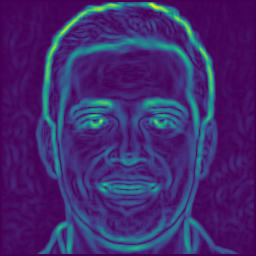
\includegraphics[width=\textwidth]{70_figures/nondd-seed1830.png}
     \end{subfigure}
     \caption{Resultant image showing the strength of the various edges after performing directional and non-directional gradient operation on the smoothened image.}
\end{figure}

The result of the operation can be visualized with the help of Fig 3.

\subsection{Weak Edge Detection}
There are several areas on facial images with curved borders, such as the chin, ear boundaries, and overall face shape. Due to the usage of both horizontal and vertical convolution kernels, these sites often have lower gradient magnitude values. However, despite having low values for the gradient magnitude, these points frequently have local maxima in both the horizontal and vertical directions because the intensity change is divided into these two directions. We take advantage of this trait to locate the curve's weak edge spots.

Therefore, we must compute a suitable lower threshold value in order to identify weak edge points. Typically, the image's Magnitude's Root Mean Square (RMS) value may be used to calculate automated threshold [6](Refer Literature Survey). The squared gradient image's mean is directly proportional to the root mean square of the image's magnitude. As a result, we base the lower threshold value on the gradient magnitude matrix's average values. The solution to equation (5) is this.

\begin{equation}
    \tau =\ 2.20\Bigg[\frac{\sum_{i}^{n}\nabla{f_i}}{n}\Bigg]
\end{equation}

$n$ denotes the gradient matrix's total number of points. If a point has local maxima in both the horizontal and vertical directions and the gradient magnitude there exceeds the lower threshold value, the point is considered to be a weak edge point.

\begin{figure}
     \centering
     \begin{subfigure}[b]{0.2\textwidth}
         \centering
         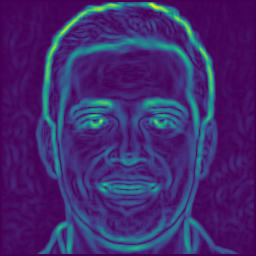
\includegraphics[width=\textwidth]{70_figures/nondd-seed1830.png}
     \end{subfigure}
     \begin{subfigure}[b]{0.2\textwidth}
         \centering
         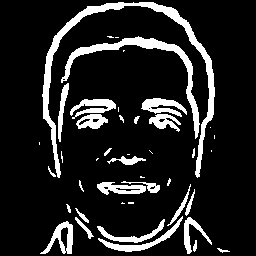
\includegraphics[width=\textwidth]{70_figures/wem-seed1830.png}
     \end{subfigure}
     \caption{Resultant image obtained after obtaining all the weak edges present.}
\end{figure}

The result of the operation can be visualized with the help of Fig 4.

\subsection{Strong Edge Detection}
Utilising composite gradient variation measures, the edge detection technique pulls out the strongest edge points from an image. By taking into account the cumulative gradient change in one direction relative to the other, composite gradient variation measurements are generated.

Each point in the image is initially represented as a function in the gradient magnitude matrix in order to find strong edge locations. A point is referred to as a strong horizontal edge point if the cumulative gradient magnitude change from one pixel to the next in the vertical direction is greater than that in the horizontal direction. A point is considered to be a strong vertical edge point if, similarly, the cumulative gradient magnitude change from one pixel to the next in the horizontal direction is more than that in the vertical direction.

A point in the gradient image is qualified as a strong edge point if it satisfies the following three criteria.
\begin{itemize}
\item The gradient magnitude at the site exceeds a predetermined upper limit. We employ a threshold of 0.825.
\item There occurs a local maximum in at least one of the directions at the point.
\item In comparison to the opposite direction, the composite gradient change along the edge direction is greater.
\end{itemize}

\begin{figure}
     \centering
     \begin{subfigure}[b]{0.2\textwidth}
         \centering
         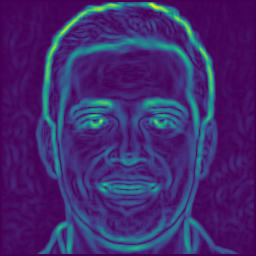
\includegraphics[width=\textwidth]{70_figures/nondd-seed1830.png}
     \end{subfigure}
     \begin{subfigure}[b]{0.2\textwidth}
         \centering
         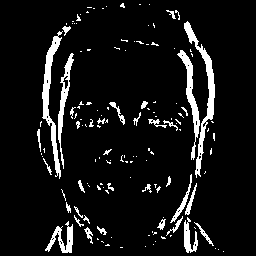
\includegraphics[width=\textwidth]{70_figures/sem-seed1830.png}
     \end{subfigure}
     \caption{Resultant image obtained after obtaining all the strong edges present.}
\end{figure}

The result of the operation can be visualized with the help of Fig 5.

\subsection{Merging}
Weak edge detection and strong edge detection techniques as discussed in sections C and D, employ thresholds, and were used to find weak and strong edges in facial images respectively. With each pixel having a value of either 0 or 1, the two techniques produce two binary images.  The output picture that exhibits both weak and strong edges is created by merging the images from the weak and strong edge detection processes.

The two pictures are combined by performing an element-wise OR operation on each corresponding pixel in the two binary images. The OR operator yields a result of 1 if either of the input pixels is 1, else a result of 0.  This produces an output image with each pixel's value set to 1 if a detected edge was found by either the weak or strong edge detection image, and to 0 otherwise.

The combined image generated by combining the two binary images acquired using the two techniques—weak edge detection and strong edge detection—is shown in Fig. 6.

\begin{figure}
     \centering
     \begin{subfigure}[b]{0.2\textwidth}
         \centering
         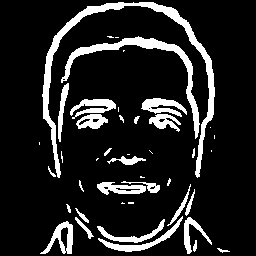
\includegraphics[width=\textwidth]{70_figures/wem-seed1830.png}
     \end{subfigure}
     \begin{subfigure}[b]{0.2\textwidth}
         \centering
         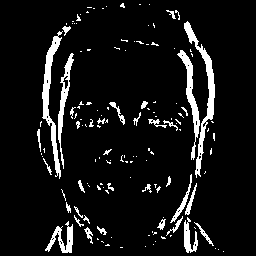
\includegraphics[width=\textwidth]{70_figures/sem-seed1830.png}
     \end{subfigure}
     \begin{subfigure}[b]{0.2\textwidth}
         \centering
         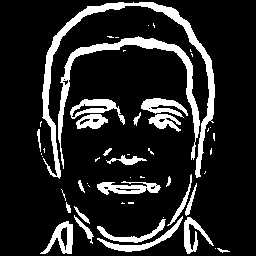
\includegraphics[width=\textwidth]{70_figures/com-seed1830.png}
     \end{subfigure}
     \caption{Resultant image obtained after combining the weak and strong edge maps.}
\end{figure}

\subsection{Thinning}
In contrast to the findings from the preceding section, the data shown in Fig. 1 reveal that the edges of a facial image are substantially thinner. The findings from the preceding section are run through the Zhang-Suen thinning \cite{6223430} method for two iterations in order to produce the edge maps seen in Fig. 1. A common technique for skeletonization, or the act of reducing a binary picture to its skeletal form, is the Zhang-Suen thinning algorithm. This technique works by repeatedly eliminating pixels from the borders of picture objects until the objects are reduced to lines that are just one pixel wide. 

\begin{figure}
     \centering
     \begin{subfigure}[b]{0.2\textwidth}
         \centering
         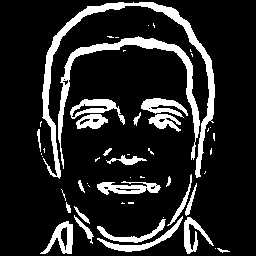
\includegraphics[width=\textwidth]{70_figures/com-seed1830.png}
     \end{subfigure}
     \begin{subfigure}[b]{0.2\textwidth}
         \centering
         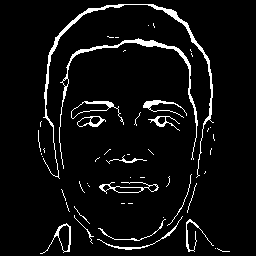
\includegraphics[width=\textwidth]{70_figures/thinned-seed1830.png}
     \end{subfigure}
     \caption{Resultant image obtained after performing the thinning operation.}
\end{figure}

The result of the operation can be visualized with the help of Fig 7.

\section{Choosing the right $\sigma$ value for smoothing}
The standard deviation parameter utilised in the Gaussian function is referred to as the $\sigma$ value of the Gaussian smoothing. It controls how much blurring or smoothing is added to the picture during the Gaussian filtering procedure.

The Gaussian function has a greater spread when the $\sigma$ value is set to a higher value. As a result, there is a greater smoothing effect since more nearby pixels are taken into account. This may be advantageous for lowering noise levels or lessening the effects of minor visual flaws. However, it could also result in the loss of certain subtle features that give the image complexity and texture.

On the other hand, the Gaussian function has a narrower spread if the $\sigma$ value is set to a lower value. As a result, the smoothing effect is less noticeable, emphasising the need of maintaining smaller features. This strategy is helpful when you want to keep the image's sharpness and clarity, but it might not be as efficient in lowering noise or minimising more significant flaws.

The distinctive features of the image, the amount of noise present, and the desired balance between maintaining details and eliminating flaws all play a role in choosing the optimal $\sigma$ value for Gaussian smoothing. It frequently calls for considerable experimentation or thorough analysis of the particular requirements of the current image processing activity. Finding the ideal setting that accomplishes the appropriate level of smoothing while preserving the crucial elements of the image is key.

\begin{table}
\centering
\begin{tabular}{|c|c|c|c|}
    \hline
    $\sigma = 1$ & $\sigma = 2$ & $\sigma = 3$ & $\sigma = 4$ \\
    \hline
    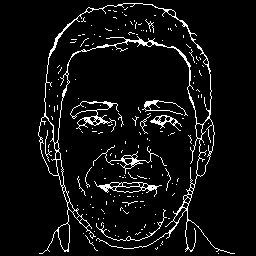
\includegraphics[width=0.2\textwidth, height=30mm]{70_figures/thinned_sigma1-seed1830.png} &
    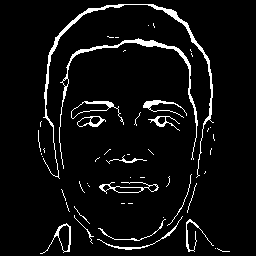
\includegraphics[width=0.2\textwidth, height=30mm]{70_figures/thinned-seed1830.png} &
    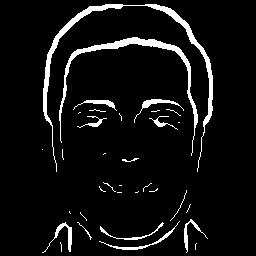
\includegraphics[width=0.2\textwidth, height=30mm]{70_figures/thinned_sigma3-seed1830.png} &
    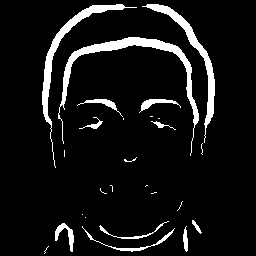
\includegraphics[width=0.2\textwidth, height=30mm]{70_figures/thinned_sigma4-seed1830.png} \\
    \hline
\end{tabular}
\caption{Comparison on results obtained from choosing different $\sigma$ values.}
\end{table}


To provide a comprehensive evaluation of the proposed algorithm's performance, a detailed comparison was conducted using Table 1 as a reference. The algorithm was tested with a range of $\sigma$ values, specifically from 1 to 4, and the results were carefully analyzed.

Upon close examination, it became evident that increasing the $\sigma$ value had a noticeable impact on the resulting edge map. Higher $\sigma$ values were found to reduce the number of details present in the edges. Interestingly, $\sigma$ = 1 produced the highest number of details in the edge map, capturing fine nuances and intricacies. However, it was deemed important to strike a balance in the edge map and avoid an excessive number of low-level features. Hence, $\sigma$ = 1 was not considered as the optimal choice.

However, as we ventured into higher $\sigma$ values of 3 and 4, a noticeable decrease in the presence of low-level features became apparent. Although these higher $\sigma$ values aimed to strike a balance, they fell short in delivering the desired level of intricate details in the resulting edge map. It became evident that a compromise had to be made to attain a harmonious edge map that effectively captured both the broader aspects and the finer nuances of the image.

After an extensive process of meticulous evaluation and thoughtful experimentation, it has become evident that a $\sigma$ value of 2 holds the key to achieving an edge map that not only accentuates the low-level details but also highlights the outline of the face flawlessly. This particular value strikes a remarkable balance, delicately preserving the fine details while avoiding an excessive influx of low-level features.

The proposed algorithm embodies a deep understanding of the significance of capturing all the necessary details while upholding utmost clarity and preventing the loss of vital information. It tirelessly seeks to find that perfect equilibrium, meticulously considering both the intricate aspects and the overall structure of the image. Through a rigorous evaluation process, coupled with careful experimentation, the optimal $\sigma$ value can be discerned, paving the way for the generation of an edge map that flawlessly encapsulates the essence of the image, displaying the essential details while preserving visual clarity and cohesiveness.

\section{Performance Measurement and Evaluation}

\subsection{Performance on different database}
The Fig. 8 showcases the outcomes obtained from extracting edge maps from the primary dataset, which consists of approximately 10,000 images with a resolution of (1024, 1024). These results demonstrate that the proposed algorithm effectively captures edges. To assess the algorithm's adaptability, it was also tested on a separate dataset using the same parameter values. The secondary dataset comprises images of various resolutions and sizes, thereby presenting a more challenging scenario to evaluate the algorithm's dynamism.


\begin{figure*}
     \centering
     \begin{subfigure}[H]{0.2\textwidth}
         \centering
         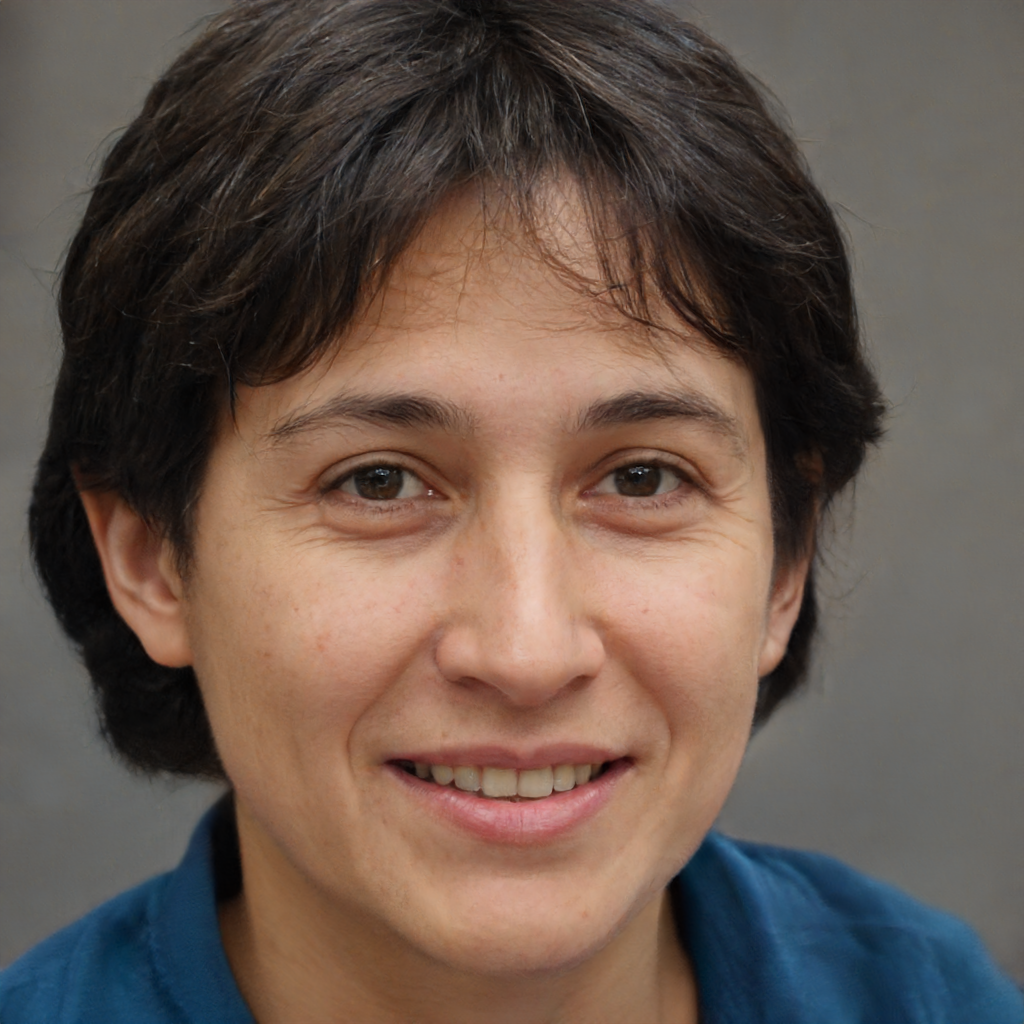
\includegraphics[width=\textwidth]{70_figures/seed7914.png}
     \end{subfigure}
     \begin{subfigure}[H]{0.2\textwidth}
         \centering
         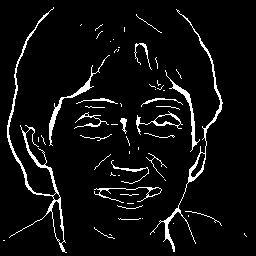
\includegraphics[width=\textwidth]{70_figures/seed7914_EM.png}
     \end{subfigure}
    \par\medskip
     \begin{subfigure}[H]{0.2\textwidth}
         \centering
         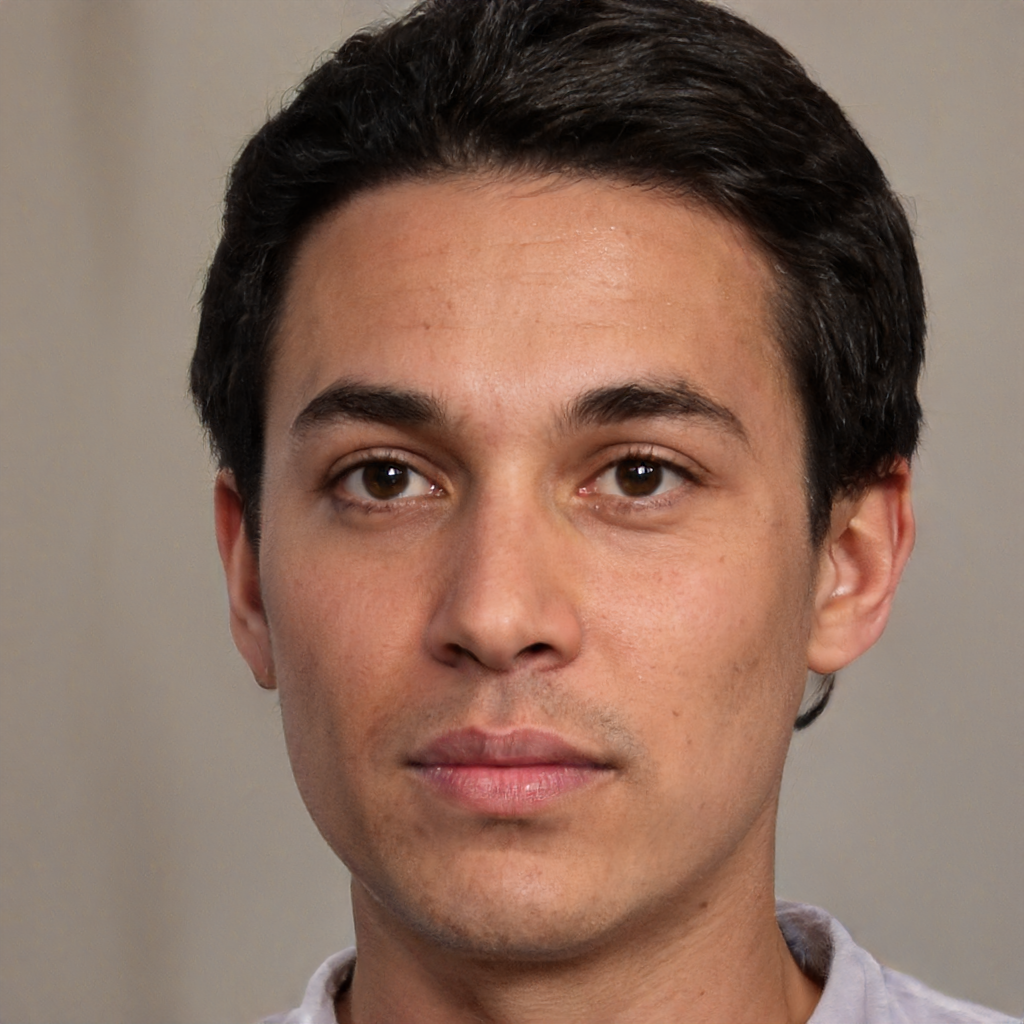
\includegraphics[width=\textwidth]{70_figures/seed7915.png}
     \end{subfigure}
     \begin{subfigure}[H]{0.2\textwidth}
         \centering
         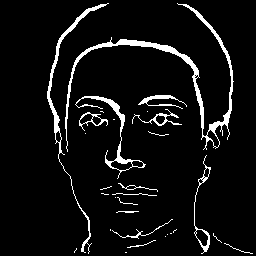
\includegraphics[width=\textwidth]{70_figures/seed7915_EM.png}
     \end{subfigure}
     \caption{Results on running the algorithm on high resolution images from the primary dataset.}
\end{figure*}

In Fig. 9, we observe the results obtained by applying the algorithm to low-resolution images. Remarkably, the proposed algorithm produces near-perfect edge maps for the low-resolution images. However, it should be noted that using low-resolution images inherently lacks fine-grained details, which subsequently affects the level of detail in the resulting edge maps. This limitation arises due to the inherent lack of detail in the low-resolution images themselves, exacerbated by the smoothing operation applied during the algorithm. Despite these constraints, the algorithm effectively generates edge maps that successfully capture the basic outlines of the low-resolution images.

\begin{figure*}
    \begin{minipage}[b]{0.47\textwidth}
        \centering
     \begin{subfigure}[H]{0.4\textwidth}
         \centering
         
\includegraphics[width=\textwidth]{70_figures/1 (79).jpg}
     \end{subfigure}
     \begin{subfigure}[H]{0.4\textwidth}
         \centering
         
\includegraphics[width=\textwidth]{70_figures/thinned-1 (79).jpg}
     \end{subfigure}
    \par\medskip
     \begin{subfigure}[H]{0.4\textwidth}
         \centering
         
\includegraphics[width=\textwidth]{70_figures/1 (662).jpg}
     \end{subfigure}
     \begin{subfigure}[H]{0.4\textwidth}
         \centering
         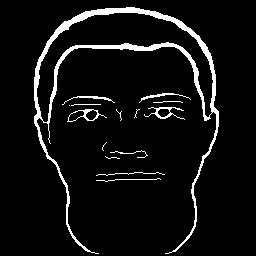
\includegraphics[width=\textwidth]{70_figures/thinned-1 (662).jpg}
     \end{subfigure}
     \caption{Results on running the algorithm on low resolution images from a different dataset.}
    \end{minipage}%
    \hspace{0.05\textwidth}
    \begin{minipage}[b]{0.47\textwidth}
        \centering
     \begin{subfigure}[b]{0.4\textwidth}
         \centering
         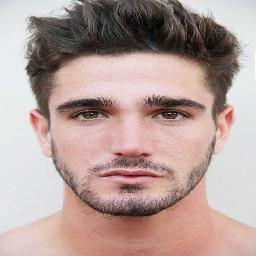
\includegraphics[width=\textwidth]{70_figures/1 (1).jpg}
     \end{subfigure}
     \begin{subfigure}[b]{0.4\textwidth}
         \centering
         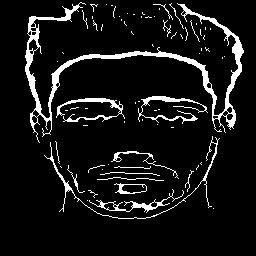
\includegraphics[width=\textwidth]{70_figures/thinned-1 (1).jpg}
     \end{subfigure}
    \par\medskip
     \begin{subfigure}[b]{0.4\textwidth}
         \centering
         
\includegraphics[width=\textwidth]{70_figures/1 (107).jpg}
     \end{subfigure}
     \begin{subfigure}[b]{0.4\textwidth}
         \centering
         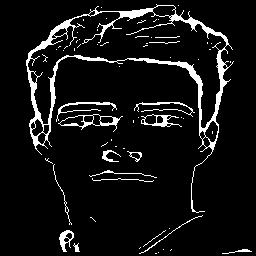
\includegraphics[width=\textwidth]{70_figures/thinned-1 (107).jpg}
     \end{subfigure}
     \caption{Results on running the algorithm on high resolution images from a different dataset.}
    \end{minipage}
\end{figure*}


Fig. 10 exhibits the outcomes of running the algorithm on high-resolution images from a different dataset. These results indicate that the algorithm is capable of extracting the fundamental outlines of the high-resolution images as well. It is important to note that since images of different resolutions possess varying levels of low-level details, the details captured in the edge maps may differ accordingly. Thus, the resulting edge maps will exhibit variations in the level of detail based on the resolution of the input images.

Overall, the findings from Figures 8, 9, and 10 collectively demonstrate the strong performance of the proposed algorithm in effectively capturing edges across different datasets and resolutions.

\subsection{Comparative Analysis}
The main objective is to present a technique for extracting an edge map from images with a high resolution, with the goal of creating an accurate edge map with fine features while preserving a balance by avoiding too many low-level information. Furthermore, it is critical that the edge map accurately and clearly depicts the the images' contours. The proposed method aims to produce an edge map that captures fine details, reduces clutter, and presents a clear depiction of the picture's outline by utilizing advanced edge detection algorithms, multi-scale techniques, noise reduction strategies, and post-processing steps.

There are several techniques available for removing edges from images. The Canny edge detection and HED (Holistically-Nested Edge Detection) algorithms are prominent options among these techniques. However, these approaches might not consistently produce encouraging outcomes when it comes to attaining the particular objective at hand. As a result, a thorough comparison study in this section has been presented that tries to draw attention to the contrasts between these well-known methodologies and our suggested method. By performing this study, we want to demonstrate the special benefits and exceptional performance of our approach, offering insightful information and supporting proof of its efficacy for edge extraction with respect to the stated objective.

A common method for edge identification in digital images is the Canny edge detection algorithm, which was created by John F. Canny in 1986. In order to get the best edge detection while minimizing noise and false detections, it takes multiple procedures. This process involves the use of Gaussian smoothing to reduce noise, gradient computation to establish the strength and direction of edges, non-maximum suppression to achieve thin edges, double thresholding to distinguish between strong and weak edges, and edge tracking using hysteresis to connect and finish edge contours.

Another sophisticated edge detection methodology that makes use of deep learning methods is the HED (Holistically-Nested Edge Detection) algorithm, which was developed by S. Xie and Z. Tu in 2015. The HED technique captures multi-scale information from the input picture using a deep convolutional neural network (CNN), collecting hierarchical representations of edges. The picture is scaled up into several sizes, features are extracted using CNN, edge maps are created at each scale, and then these maps are combined to create the final edge map. 

As we carefully examine Fig. 11, it becomes evident that there are several notable findings we can draw. The Canny edge detection algorithm, despite its widespread usage, presents certain drawbacks specifically when applied to facial images. It struggles to accurately represent the strength of the facial outline, resulting in edges that are not as robust as desired. Moreover, these edges often lack continuity, appearing fragmented and disconnected \cite{1990ph...book.....L}. Consequently, the overall depiction of the facial structure may seem incomplete or distorted, failing to capture the true essence of the face.

On the other hand, if we look at the HED (Holistically-Nested Edge Detection) edge detection algorithm, we can see that it performs better than Canny in terms of highlighting the facial outline. It does a commendable job in capturing the overall shape and contour of the face with improved accuracy. However, when it comes to capturing the intricate low-level details that make each person's face unique, like fine lines, texture, and subtle features, the HED algorithm falls a bit short. The edges it produces may not possess the level of precision and clarity necessary for a comprehensive representation of the face. They may lack the fine-grained details that truly showcase the individuality of each face.

Furthermore, the proposed methodology takes great care in finding a delicate equilibrium between the low-level and high-level details. It avoids going overboard with the emphasis on low-level details, as an excessively intricate representation could potentially compromise the overall quality and coherence of the image. Striking this balance is crucial. It allows the proposed methodology to achieve a holistic representation of the facial image, capturing both the subtle nuances and the broader aspects of the face.

To summarize, the proposed methodology goes beyond the limitations of the Canny and HED edge detection algorithms by skillfully capturing both the low-level and high-level details present in facial images. This approach ensures a comprehensive representation that boasts high resolution, resulting in a more accurate and visually pleasing depiction of the face. By considering both the intricate and broader elements of the face, the proposed methodology offers an improved and more faithful representation of facial features.

\begin{figure*}
     \centering
     \begin{subfigure}[b]{0.2\textwidth}
         \centering
         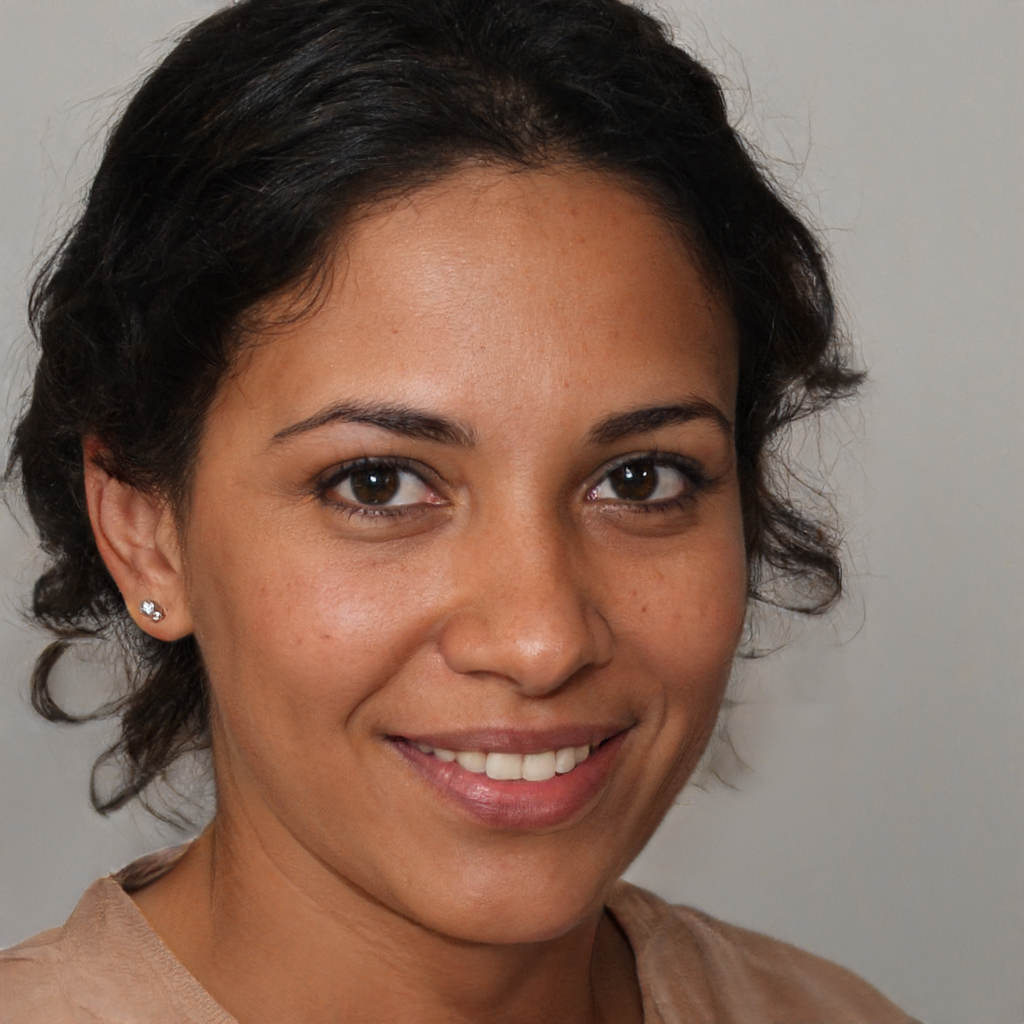
\includegraphics[width=\textwidth]{70_figures/seed0028.png}
     \end{subfigure}
     \begin{subfigure}[b]{0.2\textwidth}
         \centering
         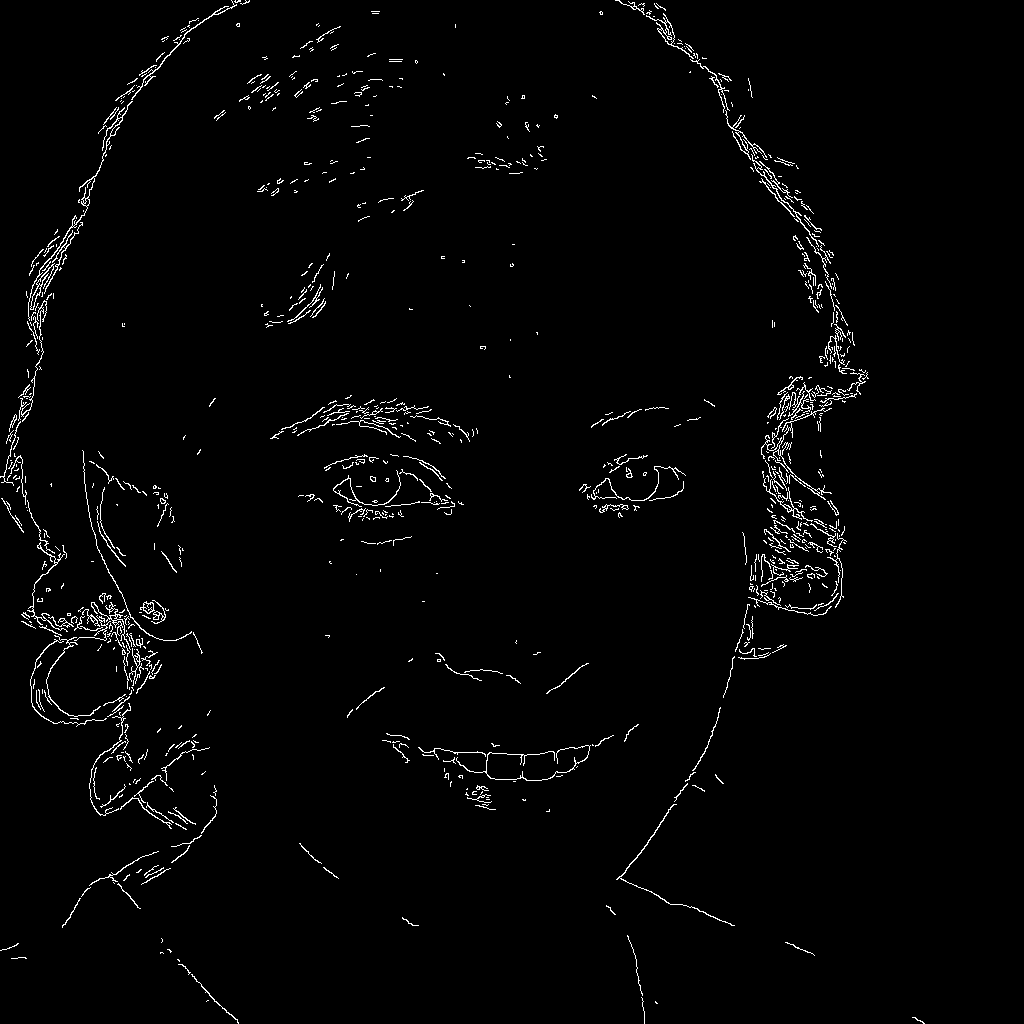
\includegraphics[width=\textwidth]{70_figures/canny-seed0028.png}
     \end{subfigure}
     \begin{subfigure}[b]{0.2\textwidth}
         \centering
         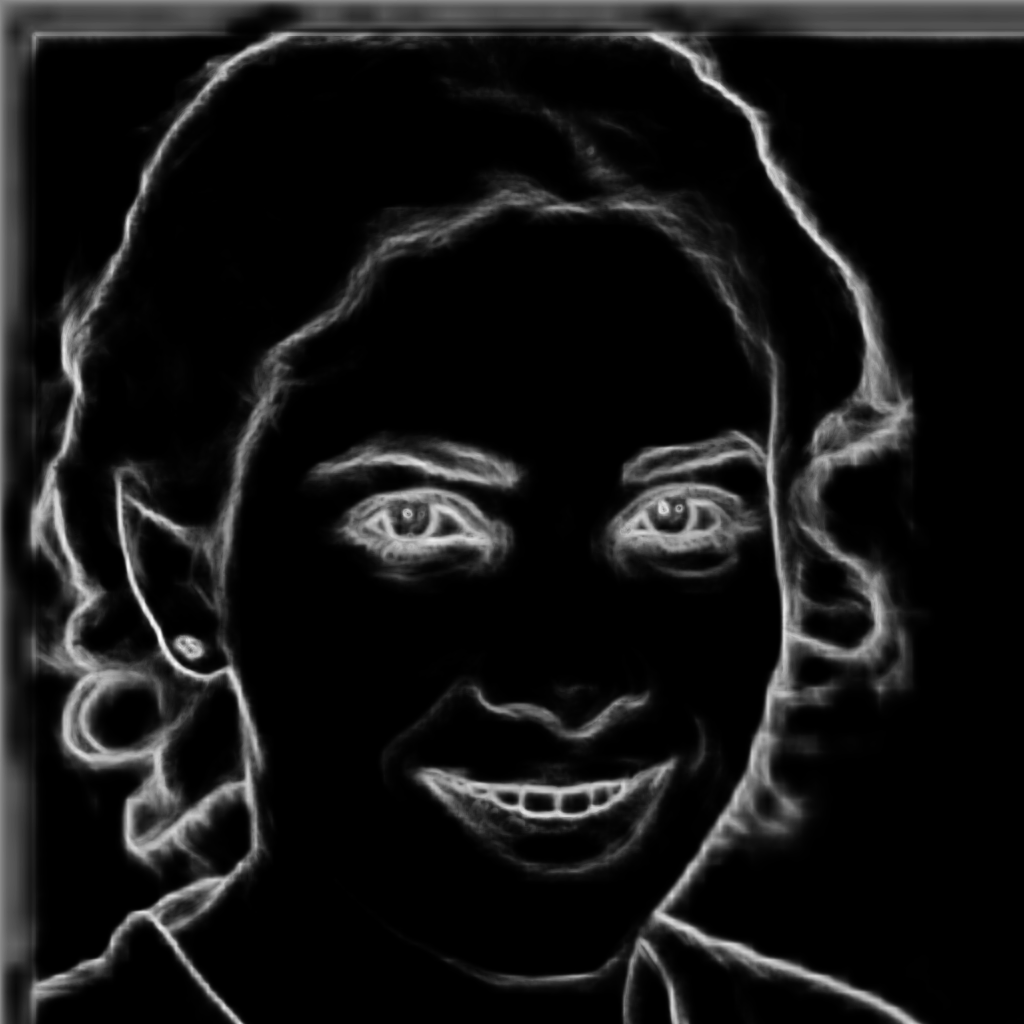
\includegraphics[width=\textwidth]{70_figures/HED_seed0028.png}
     \end{subfigure}
     \begin{subfigure}[b]{0.2\textwidth}
         \centering
         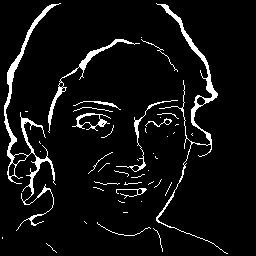
\includegraphics[width=\textwidth]{70_figures/seed0028_EM.png}
     \end{subfigure}
    \par\medskip
    \begin{subfigure}[b]{0.2\textwidth}
         \centering
         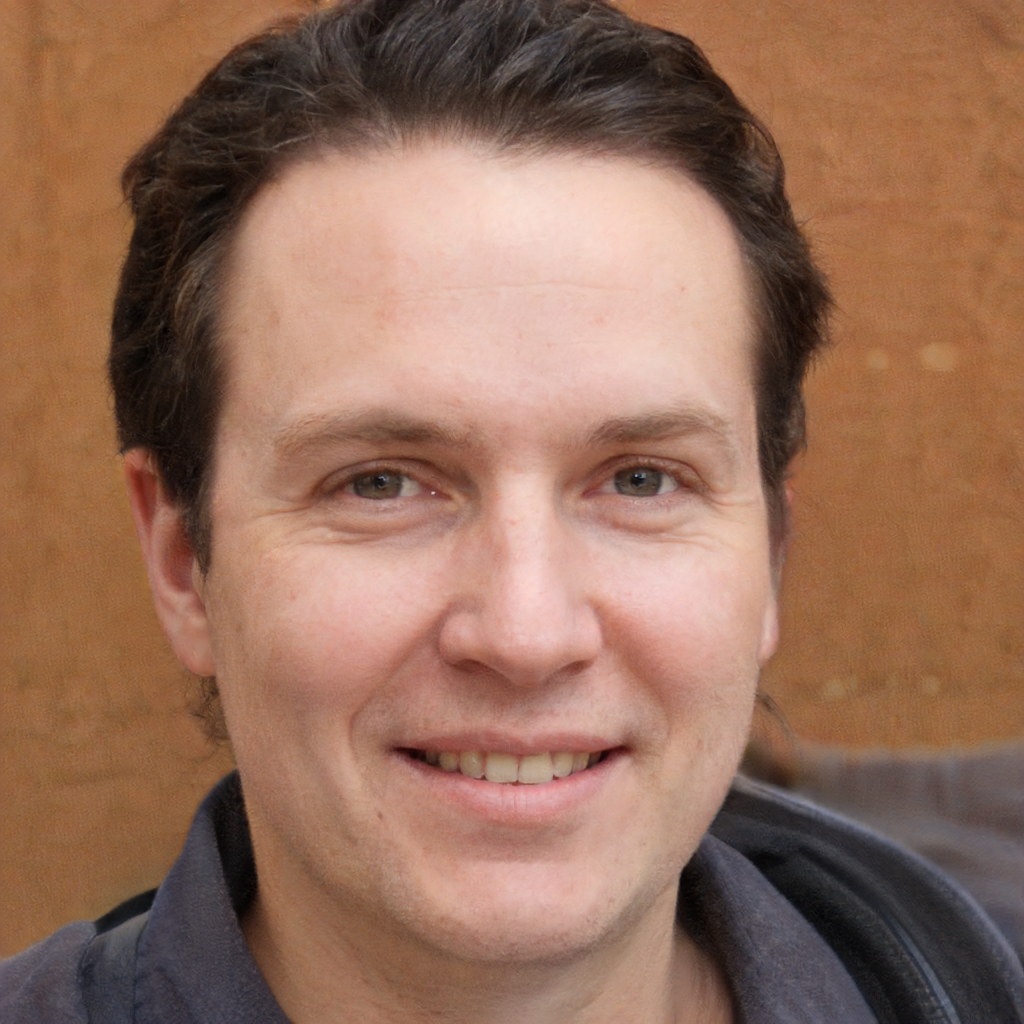
\includegraphics[width=\textwidth]{70_figures/seed0039.png}
     \end{subfigure}
     \begin{subfigure}[b]{0.2\textwidth}
         \centering
         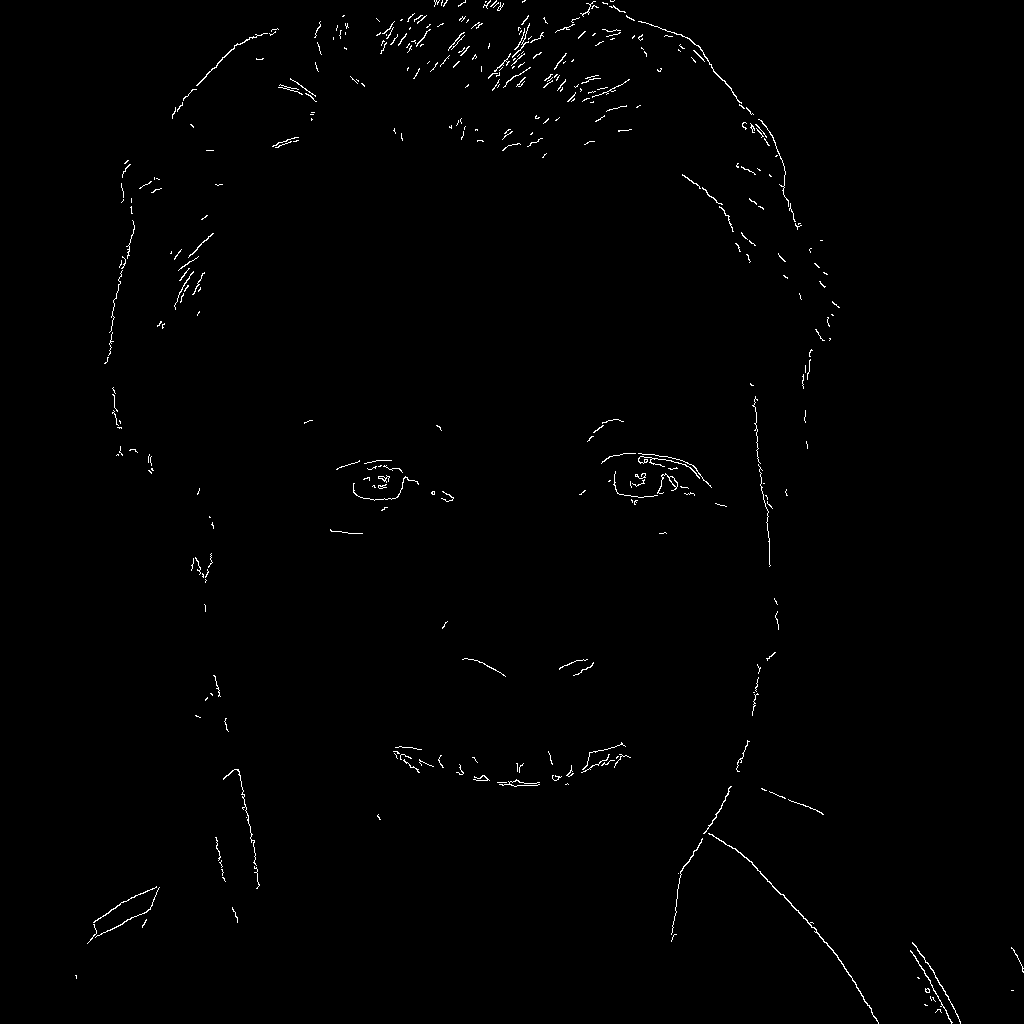
\includegraphics[width=\textwidth]{70_figures/canny-seed0039.png}
     \end{subfigure}
     \begin{subfigure}[b]{0.2\textwidth}
         \centering
         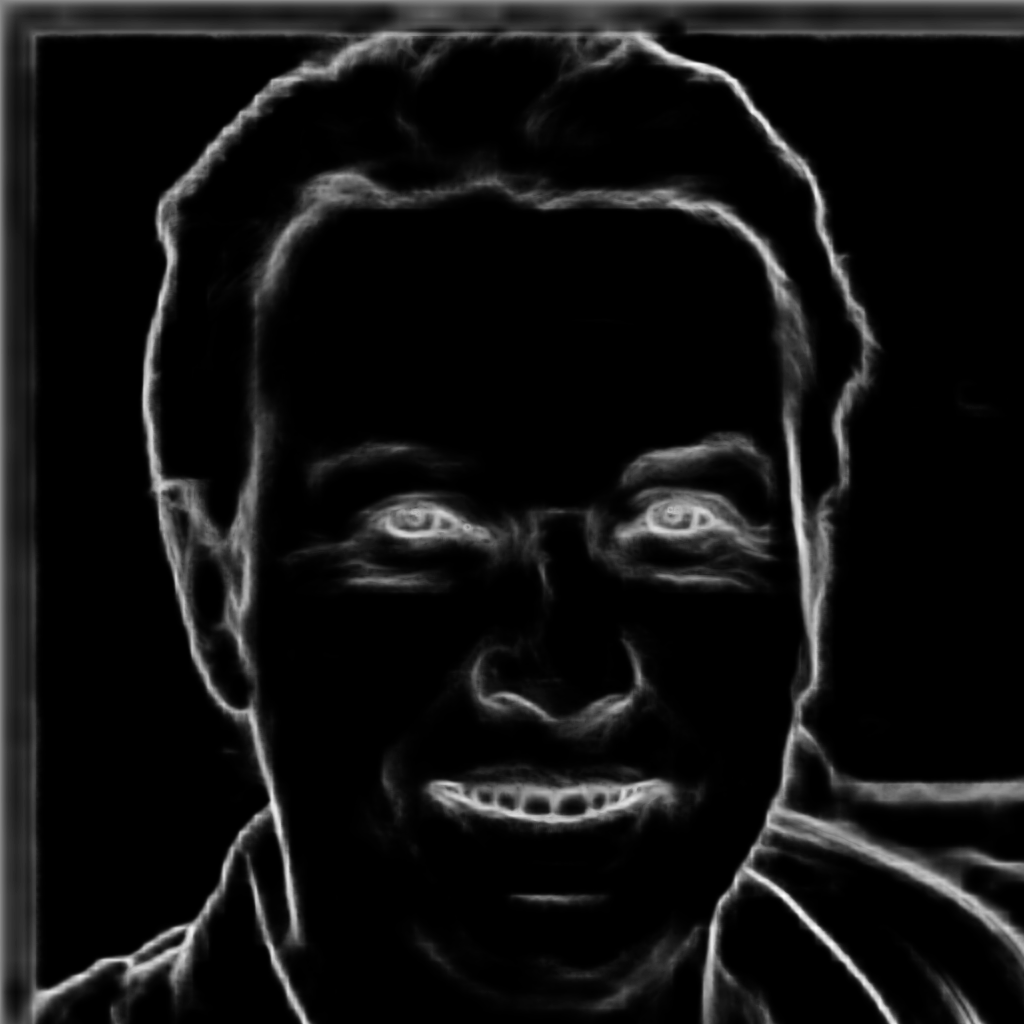
\includegraphics[width=\textwidth]{70_figures/HED_seed0039.png}
     \end{subfigure}
     \begin{subfigure}[b]{0.2\textwidth}
         \centering
         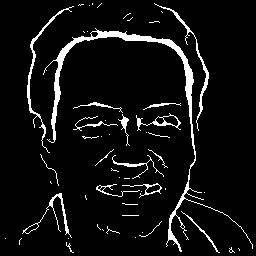
\includegraphics[width=\textwidth]{70_figures/seed0039_EM.png}
     \end{subfigure}
     \par\medskip
     \begin{subfigure}[b]{0.2\textwidth}
         \centering
         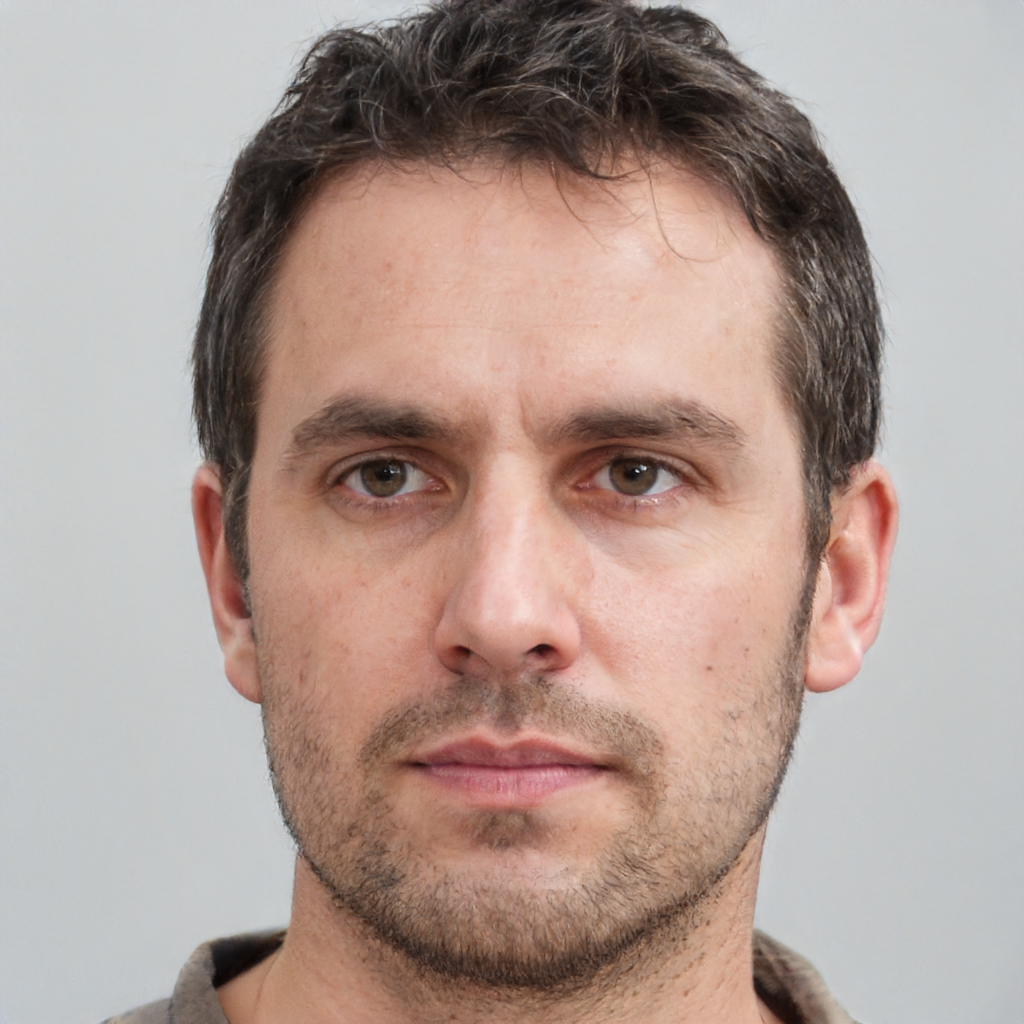
\includegraphics[width=\textwidth]{70_figures/seed0049.png}
     \end{subfigure}
     \begin{subfigure}[b]{0.2\textwidth}
         \centering
         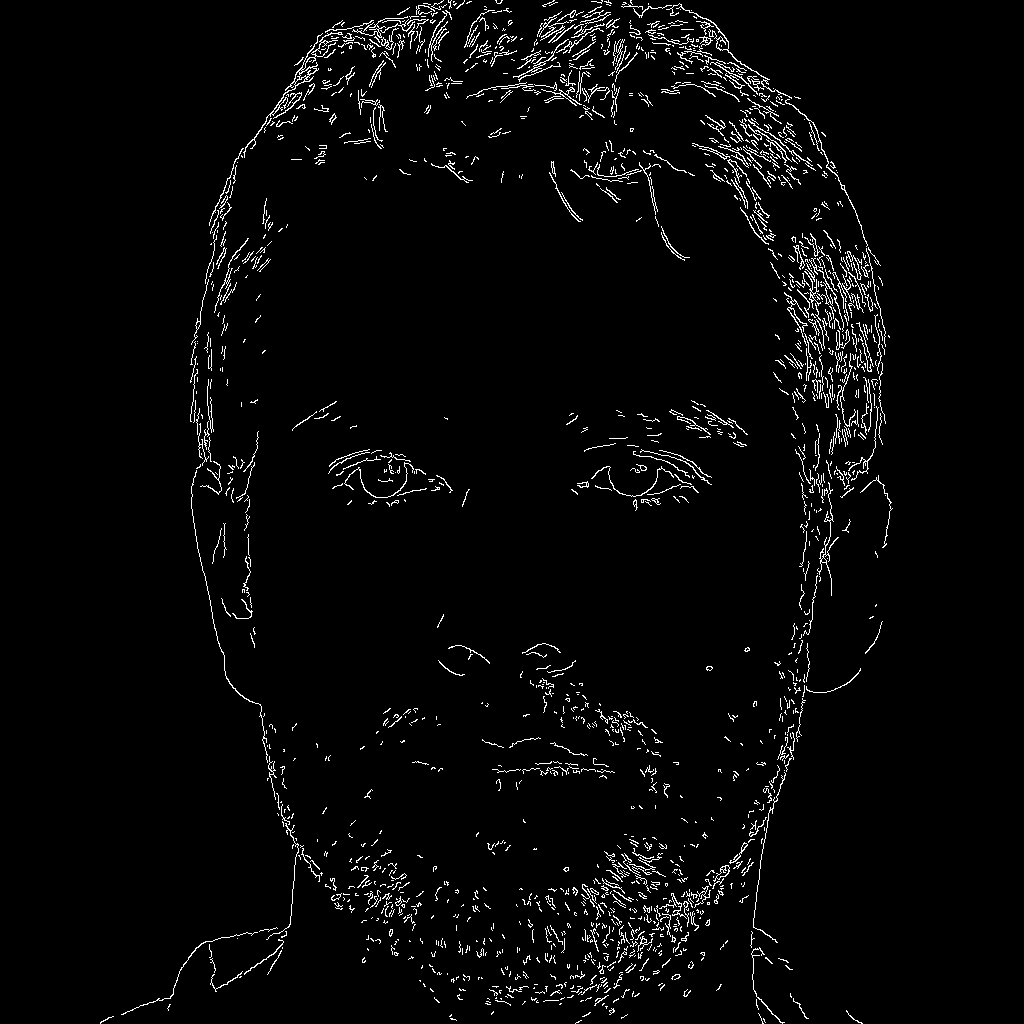
\includegraphics[width=\textwidth]{70_figures/canny-seed0049.png}
     \end{subfigure}
     \begin{subfigure}[b]{0.2\textwidth}
         \centering
         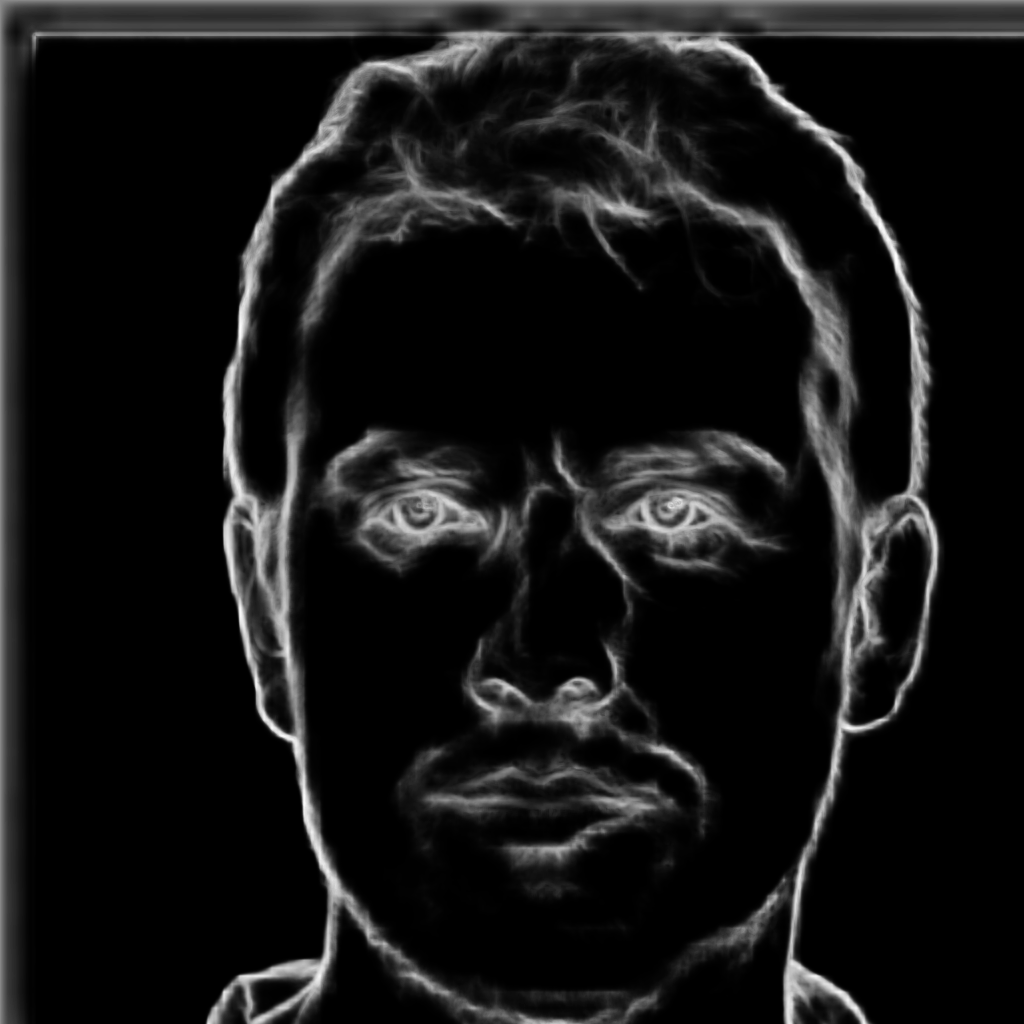
\includegraphics[width=\textwidth]{70_figures/HED_seed0049.png}
     \end{subfigure}
     \begin{subfigure}[b]{0.2\textwidth}
         \centering
         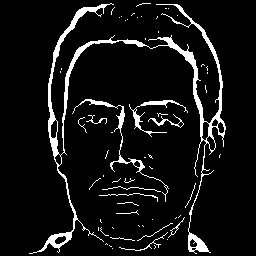
\includegraphics[width=\textwidth]{70_figures/seed0049_EM.png}
     \end{subfigure}
     \par\medskip
     \begin{subfigure}[b]{0.2\textwidth}
         \centering
         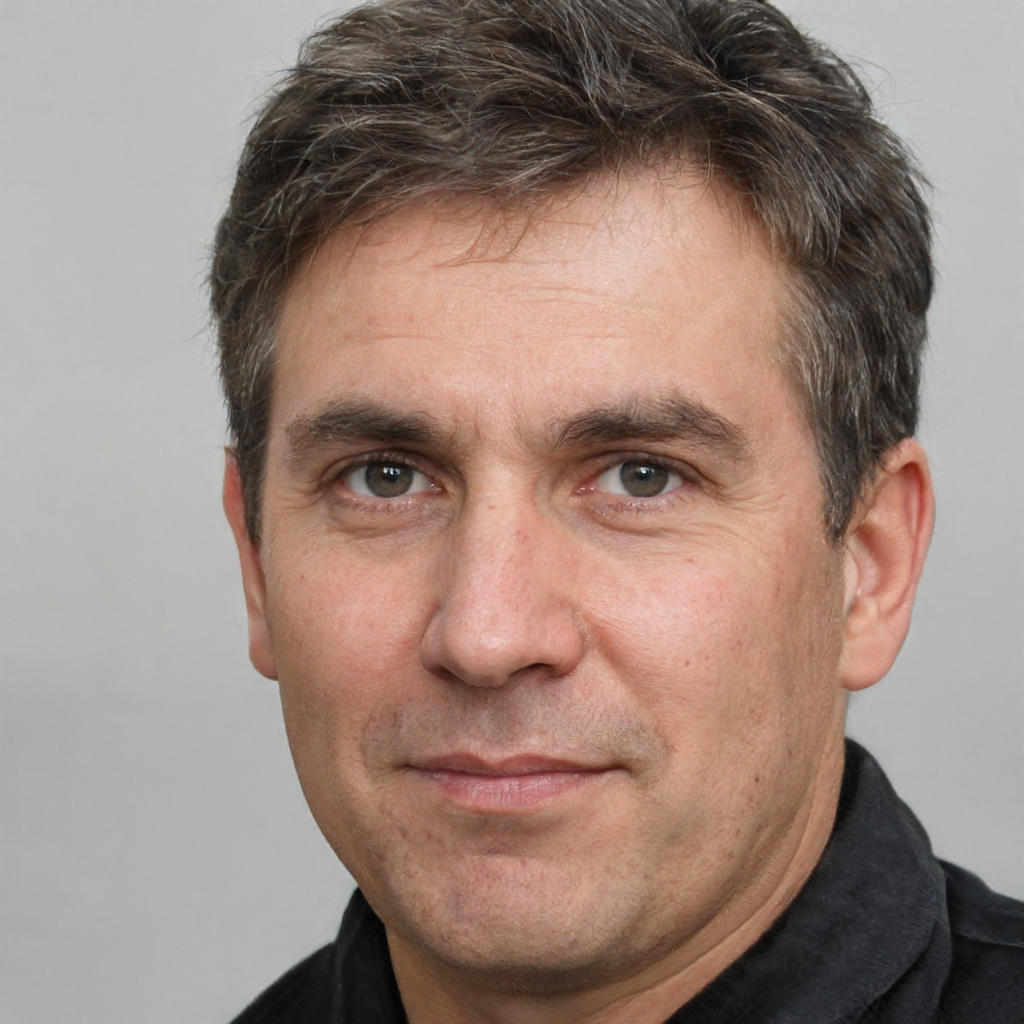
\includegraphics[width=\textwidth]{70_figures/seed0154.png}
         \caption{Original}
     \end{subfigure}
     \begin{subfigure}[b]{0.2\textwidth}
         \centering
         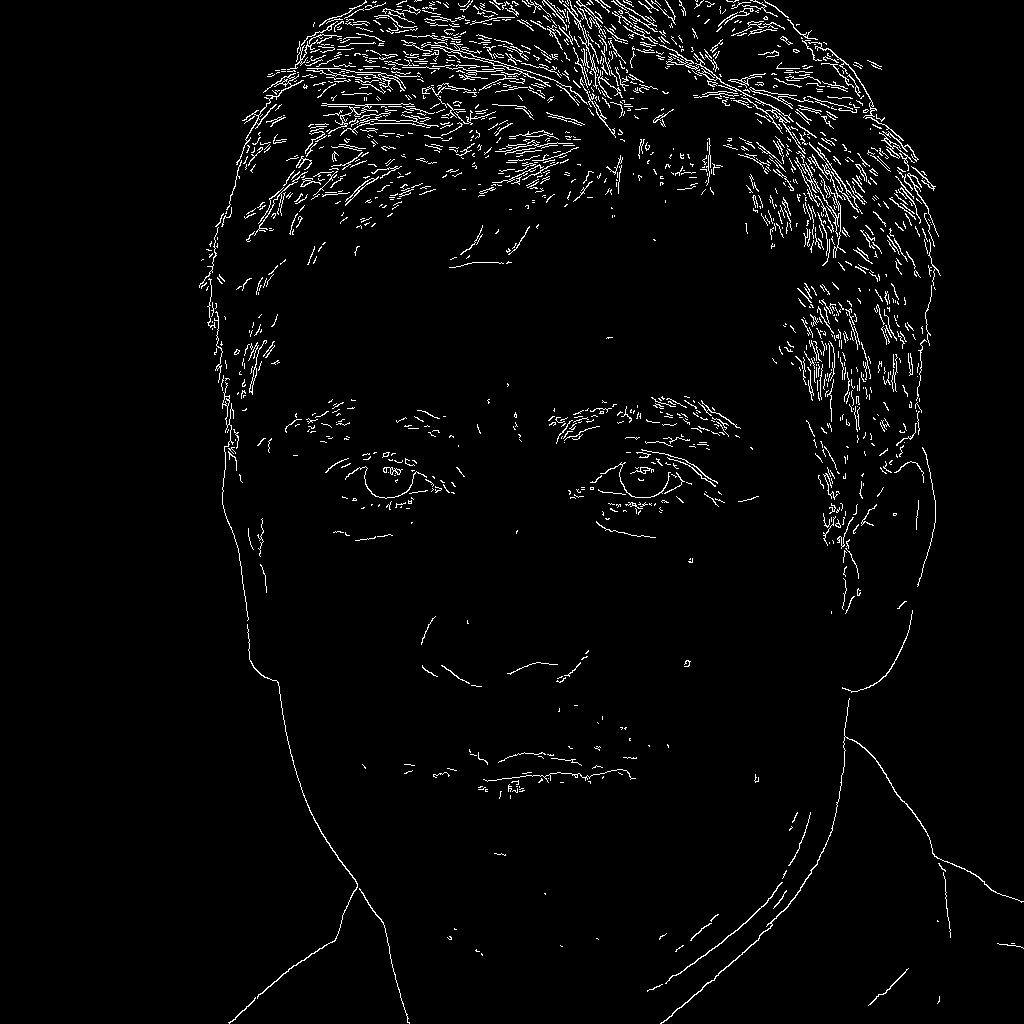
\includegraphics[width=\textwidth]{70_figures/canny-seed0154.png}
         \caption{Canny}
     \end{subfigure}
     \begin{subfigure}[b]{0.2\textwidth}
         \centering
         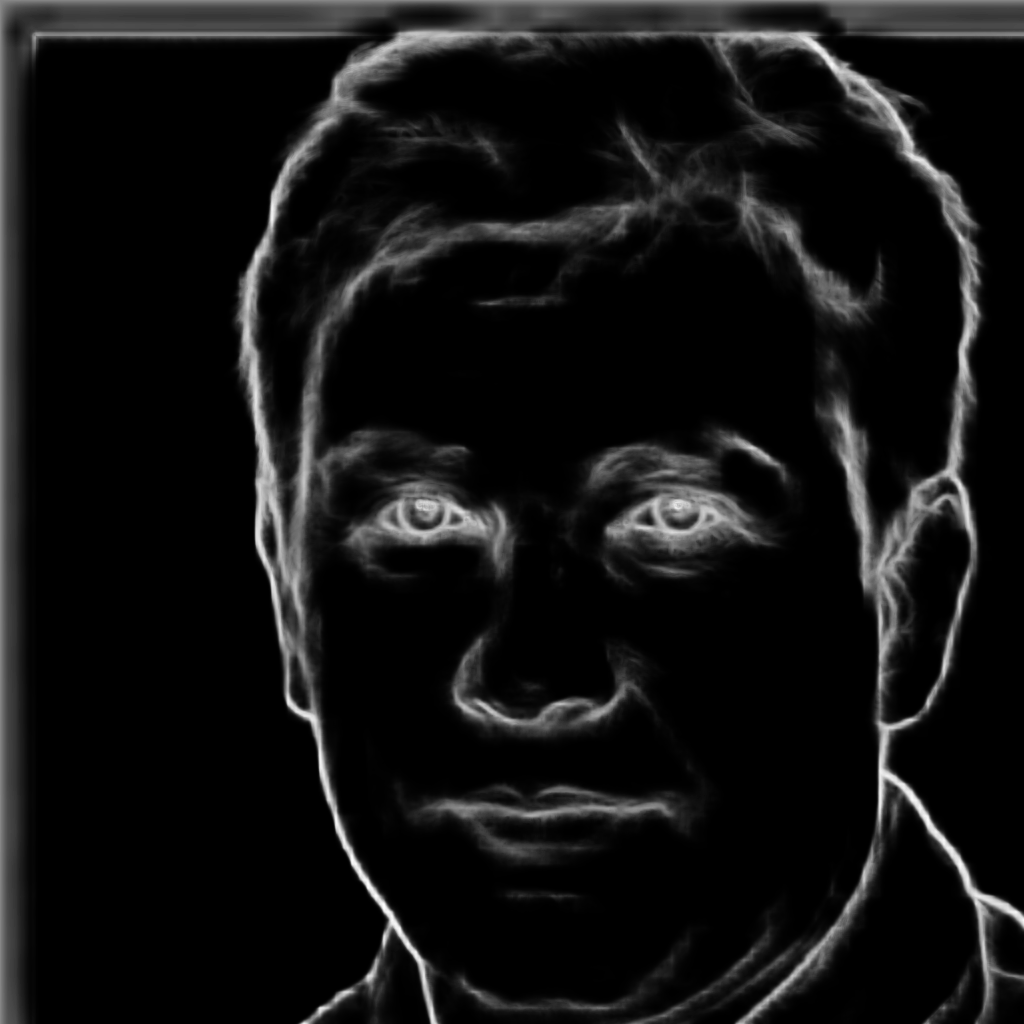
\includegraphics[width=\textwidth]{70_figures/HED_seed00154.png}
         \caption{HED}
     \end{subfigure}
     \begin{subfigure}[b]{0.2\textwidth}
         \centering
         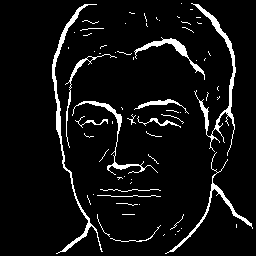
\includegraphics[width=\textwidth]{70_figures/seed0154_EM.png}
         \caption{Proposed}
     \end{subfigure}
     \caption{Comparison between different edge map detection algorithms}
\end{figure*}

\subsection{Subjective Analysis}

In this section, we present a subjective analysis aimed at evaluating the effectiveness and preciseness of the proposed algorithm for edge map extraction from high-resolution facial images, as perceived by human observers. A total of 39 volunteers participated in the analysis, providing their feedback on pairs of realistic facial images and their corresponding edge maps generated by the proposed algorithm.

The majority of the reviews indicate that the edge maps have been captured well and have successfully achieved the intended goal of outlining the facial features. Participants praised the overall accuracy and quality of the extracted edge maps, acknowledging the algorithm's ability to capture the main contours and facial structure effectively.

Nevertheless, a noteworthy finding from the reviews is that while the image's outline edges were accurately captured, some participants had concerns about the preservation of minute details. When compared to the primary outlines, these details, such as the edges around the nose or subtle facial features, were occasionally thought to be less accurate or not caught as accurately.

The participants' suggestions for improving the algorithm centered around addressing challenges related to variations in illumination and capturing low-level details in facial images. They emphasized the need to enhance the algorithm's adaptability to different lighting conditions while maintaining robustness and reliability. Additionally, they recommended fine-tuning the extraction process to achieve a more accurate and precise capture of fine-grained facial features without compromising the overall quality of the edge map. Despite recognizing the inherent difficulties in striking this balance, the participants remained optimistic about the potential for further refinement and advancements in image processing techniques. These valuable insights guide future research efforts in improving the algorithm's performance in handling illumination variations and capturing intricate facial details.

Overall, the feedback from the participants underscores the importance of addressing challenges related to illumination variations and fine-level detail extraction in the algorithm. Their valuable input serves as a guide for future research and development efforts, emphasizing the need to continue exploring innovative approaches to improve the algorithm's adaptability and precision in capturing both the main contours and the intricate details of facial images.

\section{Conclusion}
The primary objective set forth was to generate highly detailed edge maps for facial images with exceptional resolution. A pioneering methodology was proposed to overcome the limitations of existing edge detection algorithms, such as Canny and HED, by effectively leveraging both high-level and low-level information. This novel algorithm places a strong emphasis on producing edge maps that exhibit a remarkable level of realism, enabling in-depth analysis of individual facial features. The comparative analysis conducted in section 4.1, involving various edge detection techniques like Canny, HED, and the proposed methodology, yields conclusive evidence that the results achieved by the proposed approach excel not only in highlighting subtle edges and outlining the image but also in striking a delicate balance between preserving low-level details and capturing strong edges. This careful equilibrium guarantees the highlighting of all significant low-level details, resulting in the creation of highly convincing edge maps. Furthermore, a subjective analysis of the results ensures that the edge maps are not only persuasive but also visually pleasing to the volunteers involved in the evaluation process. The ongoing research will further focus on extending the methodology to images taken under different illuminations and also to produce accurate edge maps for facial images captured from lateral viewpoints.

\printbibliography

\end{document}

\end{document}